
\clearpage
\section{Procurement Function}

The procurement function supports the user when it comes to managing small or big tendering procedures. The procurements module is comprised of

\begin{itemize}
\item the procurement creation,
\item the tender inspection,
\item the award procedure,
\item the award approval and
\item the contracts.
\end{itemize}

\vspace{\baselineskip}

In addition, it is possible to illustrate different work-flows:

\begin{itemize}
\item Procurements with direct award (with one or more bidders).
\item Procurements with invitation process or open procedure.
\end{itemize}

\vspace{\baselineskip}

Since the work-flows of a procurement vary from company to company or even from project to project, this module (Procurement function) is custom made and documented for the procedures of a client. In this chapter, possible procurement processes are carried out and documented by way of example.

\vspace{\baselineskip}

\textbf{Introduction :}

In order to facilitate the navigation, procurements (invitations / calls for tender), tenders, and contracts are numbered. When creating these elements, you will be required to establish the connection (which tender concerns which procurement, which contract concerns which tender). The numbering is accordingly composed:

\vspace{\baselineskip}

Procurement n. 28 with corresponding tender n. 45 will appear in the list of tenders with the number 28.45. If contract n. 31 is added in connection to these documents, it will appear in the list of contracts with the number 28.45.31. The numbers are automatically set by CUBE PA.

\subsection{Work-flow for procurement with direct award}

This work-flow can be used for procedures with one or more bidders. \\
The work-flow is comprised of the following steps:

\begin{enumerate}
\item Creating documents for the call for tender
\item Initializing the procurement
\item Uploading documents for the call for tender
\item Sending the call for tender
\item Receiving and uploading tenders
\item Establishing tender inspection logs and sending them to the decision-making body
\item Establishing a contract.
\end{enumerate}

Statuses are used for progress monitoring when working with procurements. The statuses in the following table describe a typical project progress.

\vspace{\baselineskip}

\begin{tabular}{|p{5cm}|p{9.5cm}|}    % p{9.5cm} l} %{cl}  % {|m{5.316cm}|m{9.586cm}|}
\hline
\textbf{Status} & \textbf{Who sets the status under which conditions} \\
\hline
Call for tender creation & This status is set automatically when a procurement is initialized. \\
\hline
Approved by X & You set this status once X has reviewed the call for tender. \\
\hline
Call for tender sent to invitees & You set this status when you have sent the call for tender to the tenderers (for direct award
and invitation procedures). \\
\hline
Tender inspection & You set this status once you've entered a tender. \\
\hline
Tender with X & You set this status once you've sent this tender along with its tender inspection log to X. \\
\hline
Decision position of higher order & You set this status once you've sent this tender along with its tender inspection log to X, and that it's stated in the tender inspection log, that for example a decision from a political authority is required. \\
\hline
Award made & X sets this status once the responsible project manager or a higher authority have approved the award. \\
\hline
Contract issued & X sets this status once they have sent the unsigned contract to the tenderer. \\
\hline
Signature X / Dispatch & X sets this status once they have sent the contract, signed by the tenderer, to the awarded tenderer and the general manager. \\
\hline
Procurement completed & You set this status once you've uploaded the contract. \\
\hline
\end{tabular}

\vspace{\baselineskip}

The statuses in the following table describe a discontinuation or a halt in project progress :

\vspace{\baselineskip}

\begin{tabular}{|p{5cm}|p{9.5cm}|}    % p{9.5cm} l} %{cl}  % {|m{5.316cm}|m{9.586cm}|}
\hline
\textbf{Status} & \textbf{Who sets the status under which conditions} \\
\hline
Tender(s) refused / archived & You set this status when project management decides that this tender will no longer be followed. Project management can also set this status. \\
\hline
Tender sent back for revision & You set this status when project management decided that this tender should be sent back for revision. Project management can also set this status. \\
\hline
\end{tabular}

\subsubsection{Step 1: Establishing documents for the call for tender}

You can create the documents for the call for tender using Excel and Word, or other suitable programs.

\subsubsection{Step 2: Initializing the procurement}

\begin{wrapfigure}[3]{l}{6.5cm}   % [x] Wie manche Zeile soll sich um die Grafik "brechen"
  \vspace{-35pt}      % Grundwert war 20; mit 30 schön oben beim Text ausgerichtet
  \begin{center}
    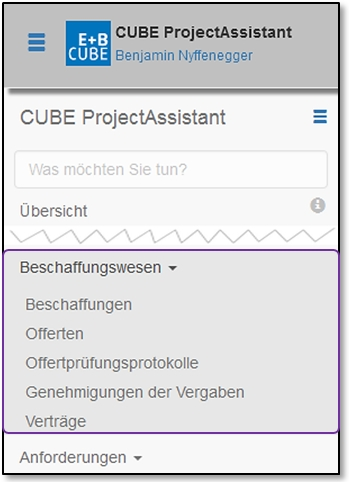
\includegraphics[width=1\linewidth]{../chapters/07_Beschaffungswesen/pictures/7-1-2_Menu_Beschaffungswesen.jpg}
  \end{center}
  \vspace{-20pt}
  \caption{Using the procurement function}
  \vspace{-10pt}
\end{wrapfigure}

In the menu on the left, select the menu item 'Procurement Function' and the sub-item 'Procurements'. 

\vspace{5cm}

The list of procurements is shown.

\vspace{2cm}

\begin{figure}[H]
\center{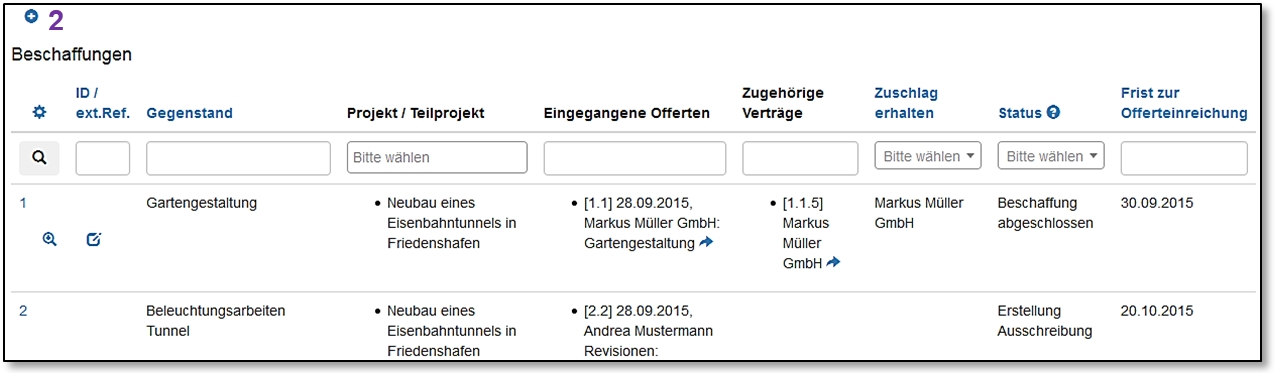
\includegraphics[width=1\linewidth]{../chapters/07_Beschaffungswesen/pictures/7-1-2_Beschaffung_Uebersicht.jpg}}
\caption{Procurements overview}
% \label{fig:speciation}
\end{figure}

% Problem

% \pagebreak
Click on the plus symbol 
\includegraphics[height=12pt]{/Icons/Plussymbol.jpg} \col{(2)} at the top left. The form for creating a new procurement appears:

\vspace{\baselineskip}

Mandatory fields are marked with an asterisk *.

\begin{figure}[H]
\center{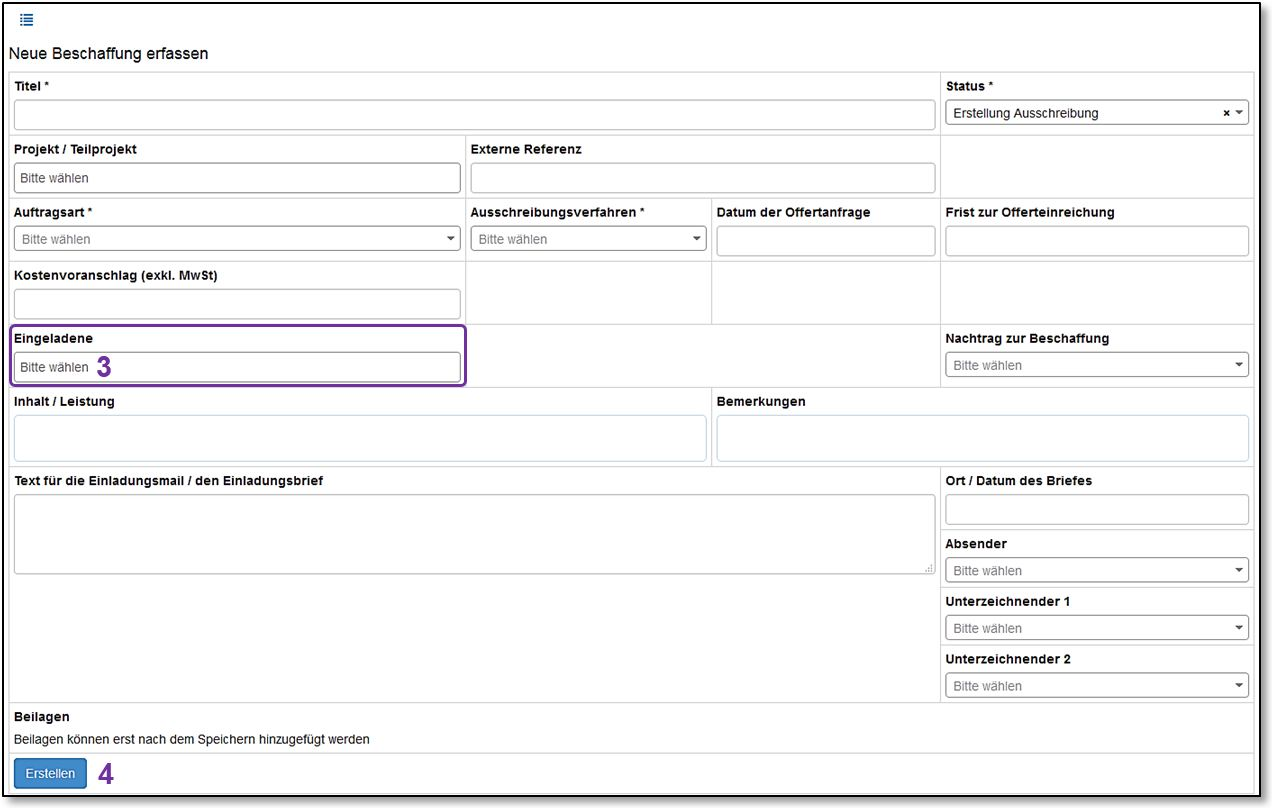
\includegraphics[width=1\linewidth]{712_BeschaffungErfassen.jpg}}
\caption{Creating a new procurement}
% \label{fig:speciation}
\end{figure}

First check if the drop-down menu of the 'Invitees' field \col{(3)} contains the company to which you want to send a call for tender. If this is not the case, switch to the 'Configuration' module in the menu on the left (see Chapter \ref{bkm:Ref434830029}) and enter the company there (Administrative rights are required for this step. Contact your CUBE PA spokesperson). If the company is in the list, select it. You can then fill out the rest of the fields:

\vspace{\baselineskip}

\begin{compactitem}
\item
Subject: Free text, short and concise.
\item
Status: Is automatically set to 'Call for tender creation' and should remain so.
\item
Project / Subproject: Select one or more corresponding project(s) / Subproject(s).
\item
External Reference: This field is only needed for retroactive logging of procurements that were in another list > not to be used.
\item
Type of order: Choose between construction contract and services contract.
\item
Tendering Procedure: Select 'Direct award'.
\item
Date of Publication: Choose the date of the tender invitation from the calendar.
\item
Deadline of Submission: Choose the deadline for receiving the tender form the calendar.
\item
Cost estimate: If there's a cost estimate, you can enter it here. You can only use numbers and one point. You will later have a direct comparison between the estimate and the tender offer.
\item
Supplementary Budget for Procurement: In case this procurement is a supplementary one for another procurement (this can be a reason why only one tenderer is written down), you can select the other procurement from the list.
\item
Content: Short description in free text of the expected services from the awarded tender, not more than 2 to 3 lines.
\item
Remarks: You can enter specific conditions for this procurement here, in later steps as well.
\item
Text for invitation mail / letter: Type the whole text of the tender invitation e-mail / letter here, with the exception of the place, time, and address. With this content, you can later generate a complete e-mail or letter invitation.
\item
If you want to send the tender invitation as a hard copy, fill out the fields 'Date, Place of Issue' (free text), 'Sender' (Drop-down selection list for the company sending the letter), 'Signature 1' (Selection list) and 'Signature 2' (Selection list). 'Signature 1' is higher in the hierarchy in case two signatures are needed.
\end{compactitem}

\vspace{\baselineskip}

Now click on the 'Create' \col{(4)}, and you can now add
attachments:

\begin{figure}[H]
\center{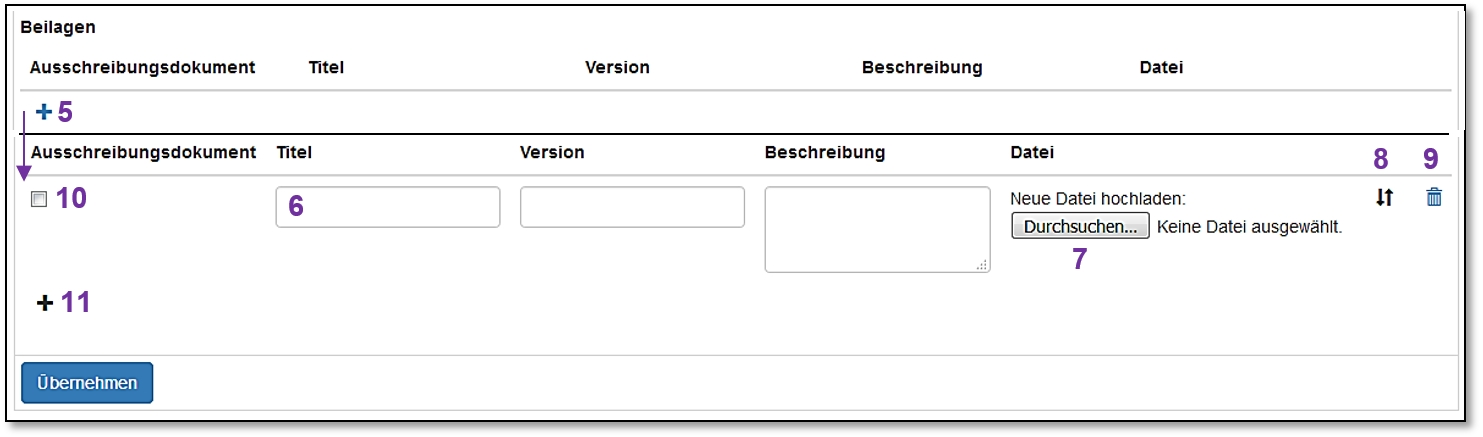
\includegraphics[width=1\linewidth]{../chapters/07_Beschaffungswesen/pictures/7-1-2_Beschaffung_Beilagen_hochladen.jpg}}
\caption{Uploading attachments to procurements}
% \label{fig:speciation}
\end{figure}

To add an attachment, click on the plus sign 
\includegraphics[height=12pt]{/Icons/Pluszeichen.jpg} \col{(5)}. You can now fill out the fields \col{(6)} and click 'Browse' \col{(7)} to upload a file. The arrows 
\includegraphics[height=12pt]{/Icons/VertPfeile.jpg} \col{(8)} allow you to change the order of an entry when you have multiple attachments (Drag and drop the arrows to place the attachment at the desired position). The garbage bin symbol 
\includegraphics[height=12pt]{/Icons/Muelltonne.jpg} \col{(9)} allows you to delete an attachment.
If you need to download the uploaded documents with the call for tender (to send the tender invitation for example), check the 'Tender Document' check-box \col{(10)}. You can add more documents using the plus symbol \includegraphics[height=12pt]{/Icons/pluszeichen.jpg} \col{(5)}. Close the process by clicking on 'Update'.

\vspace{\baselineskip}

You can now proceed immediately with step 3 or continue at a later time.

\vspace{\baselineskip}

\textbf{Intermediate step: Retroactively modifying a procurement or continuing with a procurement after an
an interruption}

\vspace{\baselineskip}

It is not necessary to proceed from step 2 to step 4 directly immediately one after the other. It is also possible to retroactively modify data after finishing a step. You can always access these steps from the procurements list. In the menu on the left, choose the 'Procurement Function' item and the 'Procurements' sub-item. The procurements list appears.

\vspace{\baselineskip}

You can visually search for a procurement within the list or filter the list to find it. To browse through the pages of the list, scroll down then use the pagination buttons to go to the next or previous page or a specific page number.

\begin{center}

\includegraphics[height=12pt]{/Icons/SeitenBlaettern.jpg}
\end{center}

To filter the list, use the search fields in the top row of the table. In the 'ID / Ext. Ref.' field, you can enter a number. The ID is the number given by CUBE PA. The 'Title' field is a free text field. The 'Project / Subproject' field is a drop-down selection list. The 'Deadline of Submission' field has a calendar selection. Once you've filled the filter fields, click on the magnifying glass symbol 
\includegraphics[height=12pt]{/Icons/Lupe_kl.jpg} \col{(1)} on the right, and the filtered list appears.

\begin{figure}[H]
\center{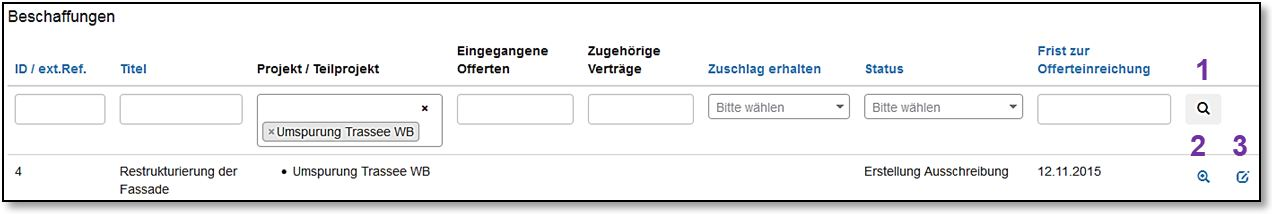
\includegraphics[width=1\linewidth]{712_BeschaffungFiltern.jpg}}
\caption{Mit dem Filter nach Geschäften suchen}
% \label{fig:speciation}
\end{figure}

Wollen Sie einen Eintrag nur ansehen, ohne ihn zu verändern, klicken Sie auf das blaue Lupensymbol 
\includegraphics[height=12pt]{/Icons/Lupe.jpg} \col{(2)}. Der Beschaffungseintrag wird geöffnet. Wenn Sie auf das Bleistiftsymbol 
\includegraphics[height=12pt]{/Icons/Bearbeiten.jpg} \col{(3)} rechts der gesuchten Zeile klicken, öffnet sich die Maske für das Bearbeiten der Beschaffung.\textcolor{red}{ }Nun können Sie entweder vorhandene Angaben korrigieren oder zu den nächsten Schritten übergehen.

\subsubsection{Schritt 3: Unterlagen für die Offertanfrage hochladen}

Nun erfassen Sie die vorab erstellten Unterlagen für die Offertanfrage als Beilagen im CUBE PA.

\vspace{\baselineskip}

Um eine Beilage zu erfassen, klicken Sie auf das Pluszeichen 
\includegraphics[height=12pt]{/Icons/Pluszeichen.jpg} \col{(1)}. Es erscheinen die Felder für eine Beilage:

\begin{figure}[H]
\center{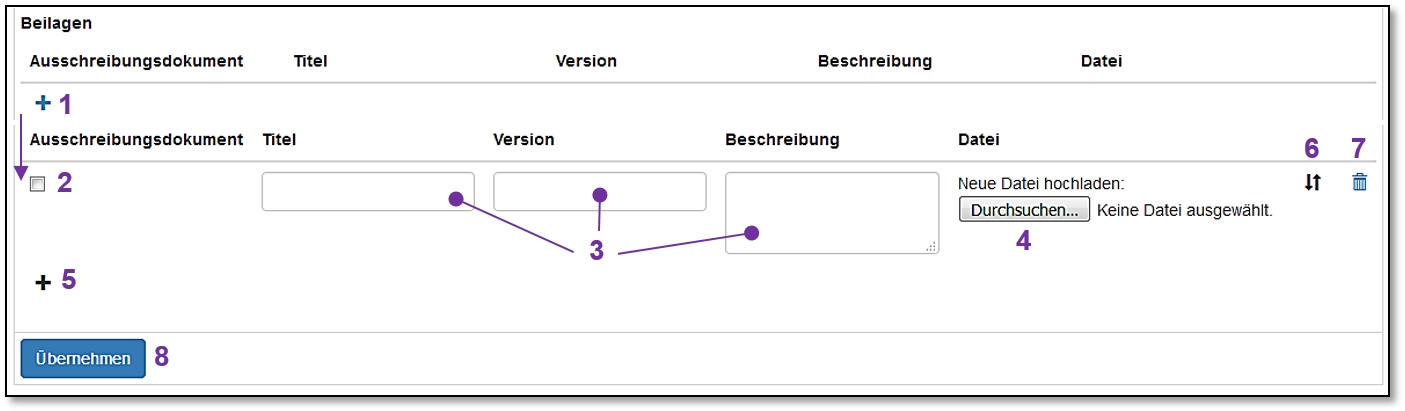
\includegraphics[width=1\linewidth]{../chapters/07_Beschaffungswesen/pictures/7-1-3_OffertanfrageHochladen.jpg}}
\caption{Eine Beilage für die Offertenanfrage hochladen}
% \label{fig:speciation}
\end{figure}

\begin{itemize}
\item Sollen die Dokumente beim Versand heruntergeladen werden können, setzen Sie ein Häkchen bei 'Ausschreibungsdokument' \col{(2)}
\item Titel, Version und Beschreibung sind freier Text \col{(3)}. In vielen Fällen wird es genügen, den Titel zu erfassen.
\item Laden Sie die Beilage hoch, indem Sie auf die Schaltfläche 'Durchsuchen' \col{(4)} klicken und eine Datei per Doppelklick auswählen. Falls Sie
eine falsche Datei gewählt haben, laden Sie einfach eine neue hoch.
\item Sie können mit dem \includegraphics[height=12pt]{/Icons/pluszeichen.jpg}-Symbol \col{(5)} weitere Beilagen hochladen.
\item Sie können die Reihenfolge der Beilagen ändern, indem Sie mit der linken Maustaste ein Symbol mit den vertikalen Pfeilen 
\includegraphics[height=12pt]{/Icons/VertPfeile.jpg} \col{(6)} packen und die Zeile verschieben.
\item Durch einen Klick auf das Mülltonnensymbol 
\includegraphics[height=12pt]{/Icons/Muelltonne.jpg} \col{(7)} können Sie eine Beilage löschen.
\item Nach dem Hochladen der Beilagen und dem Bearbeiten der Angaben (Titel etc.) schliessen Sie den Vorgang mit 'Übernehmen' \col{(8)} ab.
\end{itemize}

\textbf{Hinweis:} Der Dateiname der hochgeladenen Beialge wird automatisch im Feld 'Titel' hinzugefügt. Sie können diesen selbstverständlich anpassen.

\subsubsection{Schritt 4: Offertanfrage versenden}

In der Maske zum Bearbeiten der Beschaffung finden Sie nun oben links ein Papierflieger-Symbol 
\includegraphics[height=12pt]{/Icons/Versandsymbol.jpg}. Sobald Sie darauf klicken, erscheint die Versand-Zeile. Links steht der eingeladene Anbieter \col{(1)}, in der Mitte können Sie wiederum auf das Papierflieger-Symbol 
\includegraphics[height=12pt]{/Icons/Versandsymbol.jpg} \col{(2)} klicken, um eine E-Mail zu generieren, rechts können Sie auf das Briefsymbol 
\includegraphics[height=12pt]{/Icons/Briefsymbol.jpg} \col{(3)} klicken, um eine PDF-Datei des Briefs zu generieren, die sie nachher ausdrucken können.

\begin{figure}[H]
\center{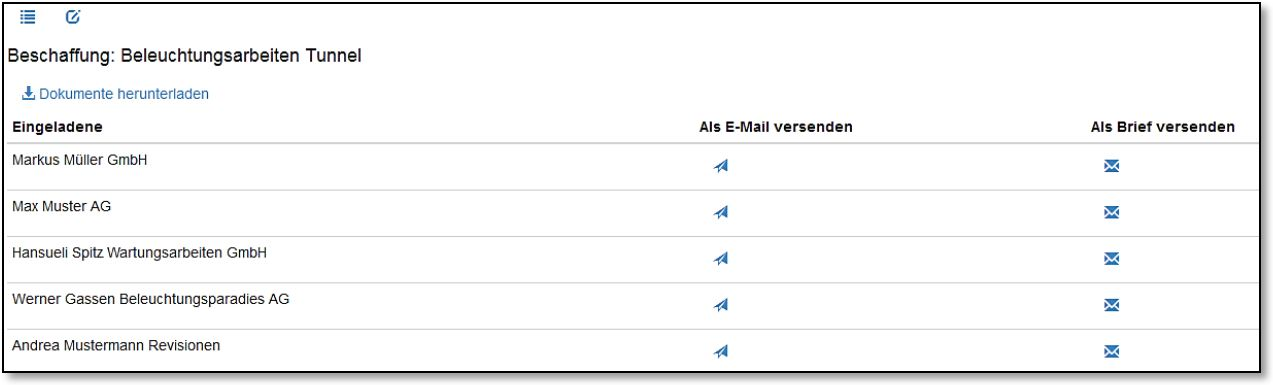
\includegraphics[width=1\linewidth]{714_BeschaffungVersand.jpg}}
\caption{Offertenanfrage versenden}
% \label{fig:speciation}
\end{figure}

Über der Versand-Zeile befindet sich eine Schaltfläche 'Dokumente herunterladen' \col{(4)} zum Herunterladen der Beilagen. Diese benötigen Sie nur, wenn Sie die Beilagen ausdrucken und dem Brief beilegen wollen.

\vspace{\baselineskip}

Wenn sie das Papierfliegersymbol 
\includegraphics[height=12pt]{/Icons/Versandsymbol.jpg} anklicken, öffnet sich die generierte E-Mail in ihrem E-Mail-Programm. Kontrollieren Sie, ob Adressat, Text und Signatur korrekt sind und nehmen Sie allfällige Korrekturen vor. Die Beilagen werden dem Mail nicht beigelegt, vielmehr erscheint ein Link, mittels dem der Empfänger die Beilagen direkt aus der Datenbank des CUBE PA herunterladen kann. Damit vermeiden Sie Probleme, die sich durch das Versenden von grossen Dateien ergeben können.

\begin{wrapfigure}[7]{r}{6cm}
\vspace{-15pt}
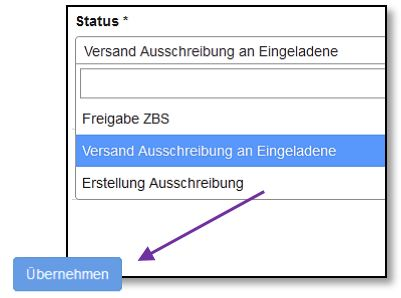
\includegraphics[height=50mm]{714_BeschaffungEingeladene.jpg}
% \caption{Status ändern}
\end{wrapfigure}

Gehen Sie zur Liste der Beschaffungen zurück (Menü links, Punkt Beschaffungswesen, Unterpunkt 'Beschaffungen', suchen Sie die Beschaffung, öffnen Sie diese zur Bearbeitung durch einem Klick auf das Bleistiftsymbol 
\includegraphics[height=12pt]{/Icons/Bearbeiten.jpg}   und setzen Sie den Status auf 'Versand Ausschreibung an Eingeladene'. Klicken Sie anschliessend auf die Schaltfläche 'Übernehmen'.

\vspace{\baselineskip}

\subsubsection{Schritt 5: Offerte entgegennehmen und hochladen}

Wählen Sie im Menü links den Punkt 'Beschaffungswesen' und den Unterpunkt 'Offerten'. Es erscheint die Liste der Offerten.

\begin{figure}[H]
\center{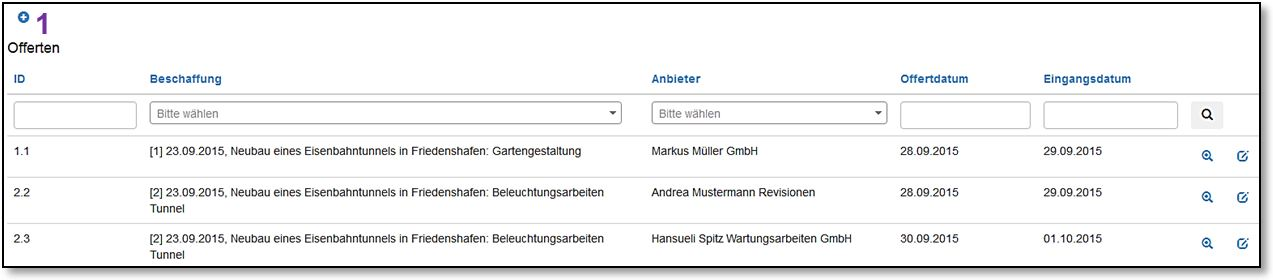
\includegraphics[width=1\linewidth]{715_OfferteUebersicht.jpg}}
\caption{Offerten Übersicht}
% \label{fig:speciation}
\end{figure}

Klicken Sie auf das Pluszeichen 
\includegraphics[height=12pt]{/Icons/Plussymbol.jpg} \col{(1)} oben links. Es erscheint die Maske für das Erfassen neuer Offerten.

\begin{figure}[H]
\center{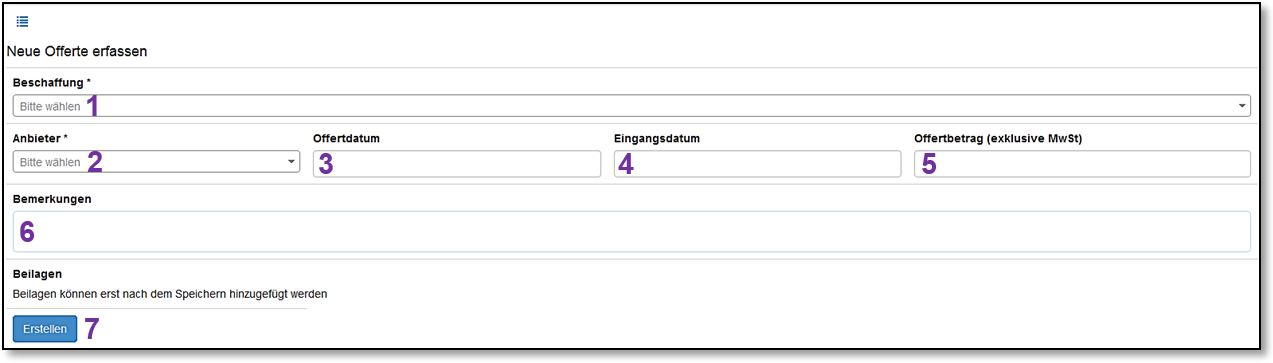
\includegraphics[width=1\linewidth]{715_OfferteErfassen.jpg}}
\caption{Neue Offerte erfassen}
% \label{fig:speciation}
\end{figure}


Mussfelder sind mit einem Stern * markiert. Füllen Sie die Felder aus:

\vspace{\baselineskip}

\begin{compactitem}
\item
Beschaffung \col{(1)}: Wählen Sie in der Liste die Offertanfrage (Beschaffung) aus, zu der die Offerte gehört. Es erscheinen nur Offertanfragen, die den Status 'Versand Ausschreibung an Eingeladene' haben.
\item
Anbieter \col{(2)}: Wählen Sie den Anbieter, der zur Offerte gehört. Wenn die Offertanfrage nur an einen Anbieter gesendet wurde, erscheint auch nur dieser Anbieter in der Liste.
\item
Offertdatum \col{(3)}: Mittels Kalenderauswahl setzen Sie das Datum ein, das auf der Offerte steht.
\item
Eingangsdatum \col{(4)}: Mittels Kalenderauswahl setzten Sie das Datum ein, an dem die Offerte eingetroffen ist.
\item
Offertbetrag \col{(5)}: Setzen Sie die Gesamtsumme der Offerte ein. Es sind nur Zahlen und ein Punkt gestattet.
\item
Bemerkungen \col{(6)}: Hier können Sie freien Text eintragen.
\end{compactitem}

\vspace{\baselineskip}

Klicken Sie nun auf die Schaltfläche 'Erstellen' \col{(7)}. Nun erscheint darunter die Möglichkeit, die Offerte
hochzuladen:

\begin{figure}[H]
\center{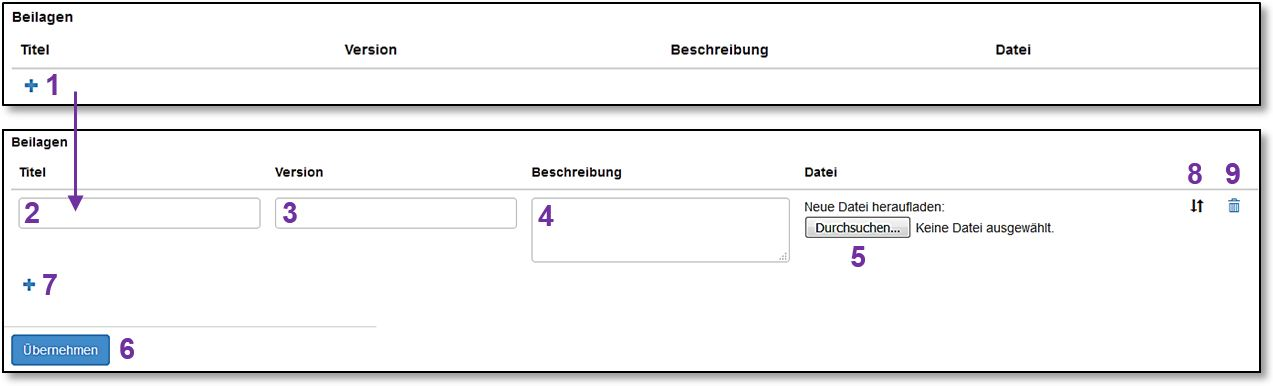
\includegraphics[width=1\linewidth]{715_OfferteHochladen.jpg}}
\caption{Offerte hochladen}
% \label{fig:speciation}
\end{figure}

Klicken Sie auf das Pluszeichen 
\includegraphics[height=12pt]{/Icons/Pluszeichen.jpg} \col{(1)}, um die Offerte hochzuladen. Erfassen Sie den Titel \col{(2)}, allenfalls auch die Version \col{(3)} und eine Beschreibung \col{(4)} des Dokuments als freien Text in den entsprechenden Feldern. Zum Hochladen klicken Sie auf die Schaltfläche 'Durchsuchen' \col{(5)} und wählen die Datei mit einem Doppelklick aus. Haben Sie eine falsche Datei erwischt, laden Sie einfach eine neue Datei hoch. Klicken Sie auf die Schaltfläche 'Übernehmen' \col{(6)} um die Daten zu sichern.

\vspace{\baselineskip}

Falls die Offerte aus mehreren Dokumenten besteht, klicken Sie wieder auf das Pluszeichen 
\includegraphics[height=12pt]{/Icons/Pluszeichen.jpg} \col{(7)} und wiederholen den Vorgang so oft wie nötig. Sie können die Reihenfolge der Dokumente verändern, indem Sie das Symbol mit den vertikalen Pfeilen 
\includegraphics[height=12pt]{/Icons/VertPfeile.jpg} \col{(8)} mit der linken Maustaste packen und die entsprechende Zeile verschieben. Mit einem Klick auf das Mülltonnensymbol 
\includegraphics[height=12pt]{/Icons/Muelltonne.jpg} \col{(9)} können Sie ein Dokument löschen.

\vspace{\baselineskip}

\begin{wrapfigure}[7]{r}{6cm}
\vspace{-15pt}
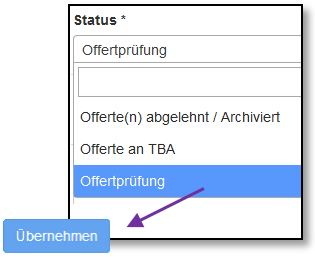
\includegraphics[height=50mm]{715_Offertpruefung.jpg}
% \caption{Status ändern}
\end{wrapfigure}
Gehen Sie in die Liste der Beschaffungen über das Menü links, Punkt 'Beschaffungswesen', Unterpunkt 'Beschaffungen'. Suchen Sie die zur Offerte gehörende Beschaffung und setzen Sie den Status auf 'Offertprüfung', in dem Sie rechts von der Zeile auf das Bleistiftsymbol 
\includegraphics[height=12pt]{/Icons/Bearbeiten.jpg} klicken und im Feld 'Status' diesen Status anwählen. Anschliessend klicken Sie auf die Schaltfläche 'Übernehmen'.

\vspace{\baselineskip}

\pagebreak
\subsubsection{Schritt 6: Offertprüfungsprotokoll erstellen und an erforderliche Stelle versenden}

\begin{wrapfigure}[7]{r}{6cm}
  \vspace{-30pt}      % Grundwert war 20; mit 30 schön oben beim Text ausgerichtet
  \begin{center}
    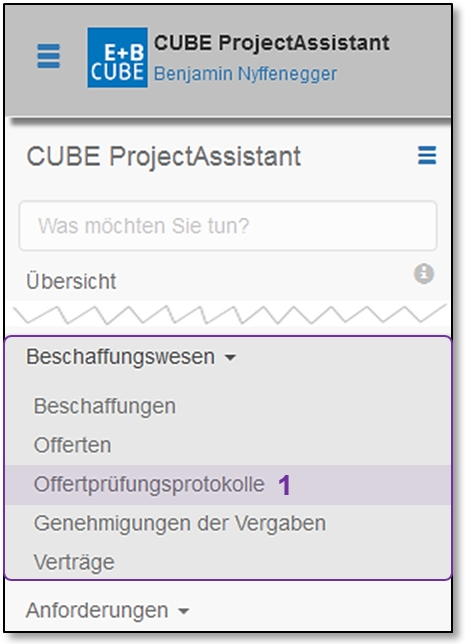
\includegraphics[height=80mm]{../chapters/07_Beschaffungswesen/pictures/7-1-6_Menu_Besch_Offertp.jpg}
  \end{center}
  \vspace{-20pt}
  \caption{Die Offertprüfungsprotokolle aufrufen}
  \vspace{-10pt}
\end{wrapfigure}

Wählen Sie im Menü links den Punkt 'Beschaffungswesen' und den Unterpunkt 'Offertprüfungsprotokolle' \col{(1)}. Es erscheint die Liste der Offertprüfungsprotokolle.

\begin{center}
\hspace{-15pt}   
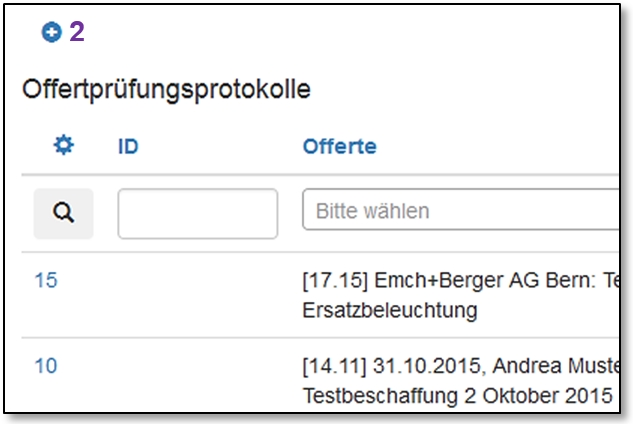
\includegraphics[width=.75\linewidth]{../chapters/07_Beschaffungswesen/pictures/7-1-6_NeuesOffertPruefProtokoll.jpg}
\end{center}

Klicken Sie auf das Pluszeichen 
\includegraphics[height=12pt]{/Icons/Plussymbol.jpg} \col{(2)} oben links. Es erscheint die Maske für das Erfassen neuer Offertprüfungsprotokolle:

\begin{figure}[H]
\center{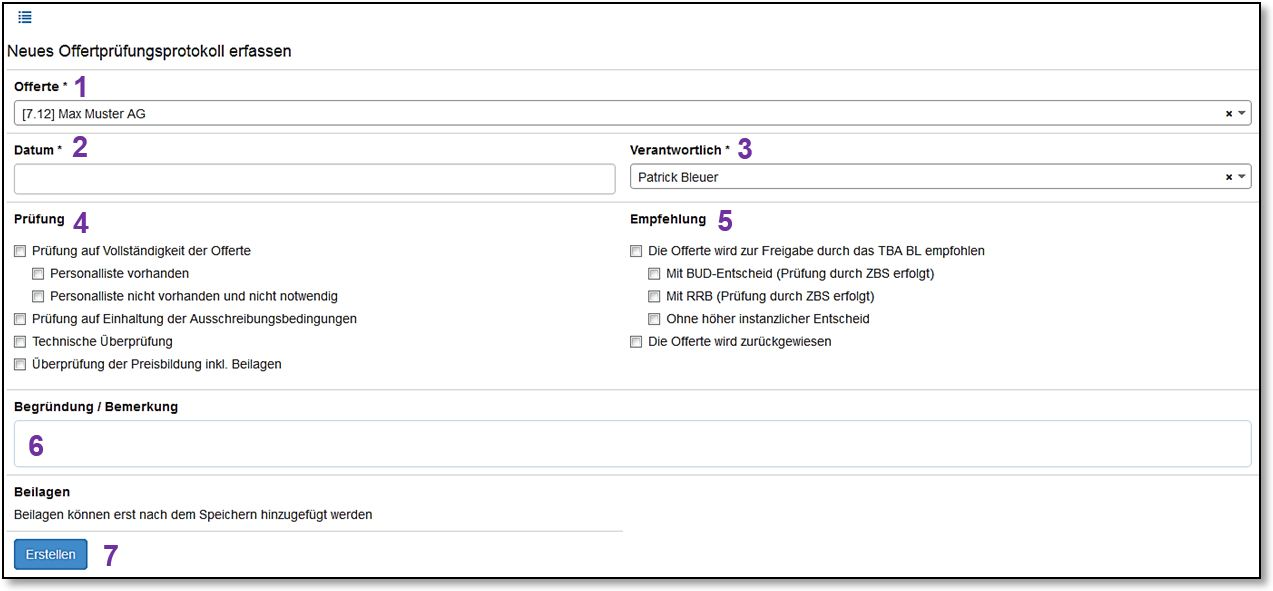
\includegraphics[width=1\linewidth]{716_OffertpruefungsprotokollErfassen.jpg}}
\caption{Neues Offertprüfungsprotokoll erfassen}
% \label{fig:speciation}
\end{figure}

Mussfelder sind mit einem Stern * markiert. Füllen Sie die Felder aus:

\vspace{\baselineskip}

\begin{compactitem}
\item
Wählen Sie im obersten Feld die zu prüfende Offerte. Die Auswahlliste \col{(1)} zeigt nur diejenigen Offerten, für die noch kein Offertprüfungsprotokoll existiert.
\item
\textcolor{black}{Datum }\col{(2)} \textcolor{black}{: Geben Sie das Datum des Offertprüfungsprotokoll an. Beim Klicken in das Datumfeld öffnet sich ein Kalender, in welchem Sie den gewünschten Tag auswählen können. }Als Default-Wert wird jeweils das heutige Datum vorgeschlagen.
\item
Wählen Sie im Feld 'Verantwortlich' \col{(3)} den Verantwortlichen für das Offertprüfungsprotokoll aus. Der Verantwortliche ist diejenige Person, die das Offertprüfungsprotokoll unterschreibt.
\item {\sffamily
Klicken Sie unter 'Prüfung' \col{(4)} und 'Empfehlung' \col{(5)} die zutreffenden Kästchen an.}
\item
Schreiben Sie im Feld 'Begründung/Bemerkung' \col{(6)} falls nötig einen freien Text.
\end{compactitem}

\vspace{\baselineskip}

Klicken Sie auf die Schaltfläche 'Erstellen' \col{(7)}. Nun erscheint darunter die Möglichkeit, eine Beilage hochzuladen.

\begin{figure}[H]
\center{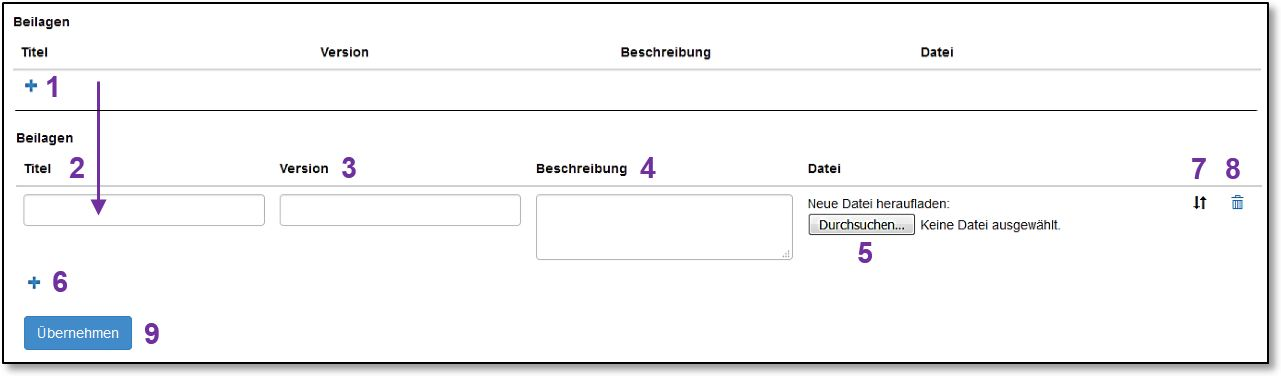
\includegraphics[width=1\linewidth]{716_OffertenpruefungsprotokollBeilagen.jpg}}
\caption{Beilage beim Offertprüfungsprotokoll hochladen}
% \label{fig:speciation}
\end{figure}

Klicken Sie auf das Pluszeichen 
\includegraphics[height=12pt]{/Icons/Pluszeichen.jpg} \col{(1)}, um die Beilage hochzuladen. Erfassen Sie den Titel \col{(2)}, allenfalls auch die Version \col{(3)} und eine Beschreibung des Dokuments \col{(4)} als freien Text in den entsprechenden Feldern. Zum Hochladen klicken Sie auf die Schaltfläche 'Durchsuchen' \col{(5)} und wählen die Datei mit einem Doppelklick aus. Haben Sie eine falsche Datei erwischt, laden Sie einfach eine neue Datei hoch. Klicken Sie auf die Schaltfläche 'Übernehmen' um die Daten zu sichern. \\
Falls es mehrere Beilagen braucht, klicken Sie wieder auf das Pluszeichen 
\includegraphics[height=12pt]{/Icons/Pluszeichen.jpg} \col{(6)} und wiederholen den Vorgang so oft wie nötig. Sie können die Reihenfolge der Dokumente verändern, indem Sie das Symbol mit den vertikalen Pfeilen 
\includegraphics[height=12pt]{/Icons/VertPfeile.jpg} \col{(7)} mit der linken Maustaste packen und die entsprechende Zeile verschieben. Mit einem Klick auf das Mülltonnensymbol 
\includegraphics[height=12pt]{/Icons/Muelltonne.jpg} \col{(8)} können Sie ein Dokument löschen.

\vspace{\baselineskip}

\begin{wrapfigure}[7]{r}{5cm}
\vspace{-15pt}
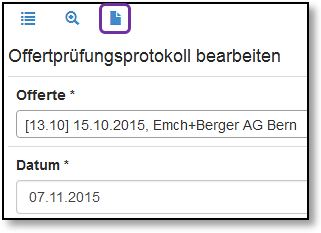
\includegraphics[height=40mm]{716_OffertpruefungsprotokollPDFgen.jpg}
% \caption{Status ändern}
\end{wrapfigure}
Klicken Sie auf 'Übernehmen' \col{(9)}, um die Daten zu sichern. Nun können Sie oben links auf das
Blatt mit der gefalteten Ecke \includegraphics[height=12pt]{/Icons/BLattsymbol.jpg} klicken, um ein Offertprüfungsprotokoll als PDF-Datei zu generieren. Drucken Sie es aus und lassen Sie es unterschreiben. Das unterschriebene Dokument wird anschliessend eingescannt und bei diesem Offertprüfungsprotokoll als
Beilage wieder angehängt. Das Offertprüfungsprotokoll (Original) wird dann zusammen mit dem Papieroriginal der Offerte an die erforderliche Stelle gesendet.

\vspace{\baselineskip}

\begin{wrapfigure}[7]{r}{6cm}
\vspace{-15pt}
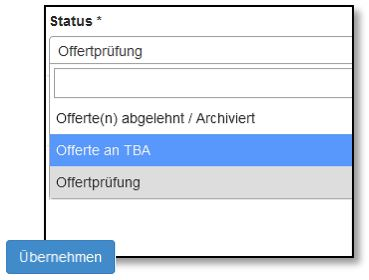
\includegraphics[height=50mm]{716_BeschaffungStatus.jpg}
% \caption{Status ändern}
\end{wrapfigure}
Gehen Sie im Menü links zum Punkt 'Beschaffungswesen', Unterpunkt 'Beschaffungen'. Suchen Sie die zur Offerte gehörende
Beschaffung und setzen Sie den Status auf 'Offerte Stelle X', in dem Sie rechts von der Zeile auf das Bleistiftsymbol 
\includegraphics[height=12pt]{/Icons/Bearbeiten.jpg} klicken und im Feld 'Status' diesen Status anwählen. Anschliessend klicken Sie auf die Schaltfläche 'Übernehmen'.

\vspace{\baselineskip}

Nun kommen Sie erst wieder zum Zug, wenn die entsprechende Stelle den Vertrag ausgestellt hat und dieser von beiden Parteien unterschrieben wurde. Der Gesamtleiter erhält eine Kopie des Vertrags und erfasst diesen im CUBE PA, damit der Vertragsinhalt zugänglich ist.

\subsubsection{Schritt 7: Genehmigung der Vergabe durch eine höhere Instanz}

Falls Sie im Offertprüfungsprotokoll angekreuzt haben, dass die Vergabe durch eine höhere Instanz (zum Beispiel Bau- und Umweltschutzdirektion oder Regierungsrat) genehmigt werden soll, setzen Sie den Status der Beschaffung auf 'Entscheid höher instanzliche Stelle'.

\subsubsection{Schritt 8: Vertrag erfassen}

\begin{wrapfigure}[7]{r}{6cm}
  \vspace{-30pt}      % Grundwert war 20; mit 30 schön oben beim Text ausgerichtet
  \begin{center}
    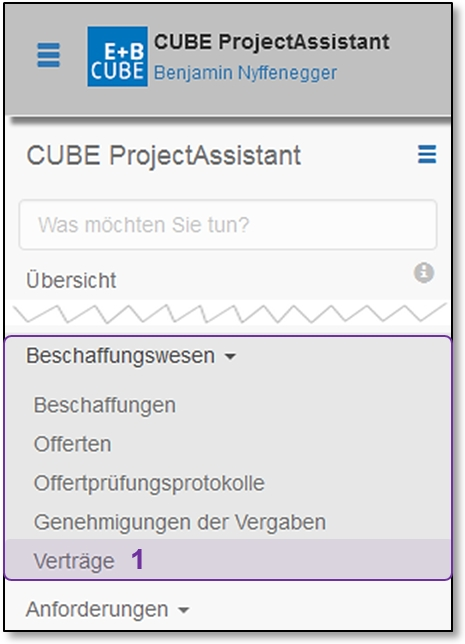
\includegraphics[height=80mm]{../chapters/07_Beschaffungswesen/pictures/7-1-8_Menu_Besch_Vertraege.jpg}
  \end{center}
  \vspace{-20pt}
  \caption{Die Adressliste im Menü aufrufen}
  \vspace{-10pt}
\end{wrapfigure}

Verträge werden sowohl in TDCost erfasst (als Grundlage für die Kostenkontrolle) als auch im CUBE PA, um den Verlauf der Beschaffung vollständig zu dokumentieren und den Inhalt des Vertrags zugänglich zu machen. Erfassen Sie den Vertrag wenn möglich zuerst in TDCost, damit Sie über alle im CUBE
PA nützlichen Angaben verfügen.

\begin{center}
\hspace{-55mm}   
\includegraphics[width=.4\linewidth]{../chapters/07_Beschaffungswesen/pictures/7-1-8_NeuerVertrag.jpg}
\end{center}

\vspace{\baselineskip}

Wählen Sie im Menü links den Punkt 'Beschaffungswesen' und den Unterpunkt 'Verträge' \col{(1)}. Es erscheint die Liste der Verträge.

\vspace{\baselineskip}

Klicken Sie auf das Plussymbol \includegraphics[height=12pt]{/Icons/Plussymbol.jpg} \col{(2)} oben links. Es erscheint die Maske für das Erfassen neuer Verträge. Mit dem Listensymbol \includegraphics[height=12pt]{/Icons/Listensymbol_zurueck.jpg} \col{(3)} können Sie zurück zur Liste / Übersicht wechseln.

\begin{figure}[H]
\center{\includegraphics[width=1\linewidth]{718_VertragErfassen.jpg}}
\caption{Neuer Vertrag erfassen}
% \label{fig:speciation}
\end{figure}

Mussfelder sind mit einem Stern * markiert. Füllen Sie die Felder aus:

\vspace{\baselineskip}

\begin{compactitem}
\item {\sffamily\color{black}
Unter 'Offerte' wählen Sie die Offerte, die als Basis zum Vertrag gedient hat. Es erscheinen nur diejenigen Offerten, die nicht zu einer abgeschlossenen Beschaffung gehören.}
\item
Der 'Vertragstitel' wird automatisch aus den Angaben zur Offerte übernommen, Sie können ihn jedoch bearbeiten.
\item
Das 'Projekt/Teilprojekt' wird automatisch aus den Abgaben zur Beschaffung übernommen. Sie können jedoch die Auswahl ändern oder ergänzen.
\item
Das 'Vertragsdatum' können Sie über eine Kalenderauswahl setzen.
\item
Das 'Startdatum' und das 'Enddatum' werden ebenso über eine Kalenderauswahl gesetzt. Es handelt sich dabei um die Termine, an denen die Leistungserbringung beginnen und enden soll.
\item
Den 'Auftraggeber' wählen Sie aus einer Auswahlliste, der 'Auftragnehmer' erscheint automatisch aufgrund der Angaben zur Offerte.
\item
Auch die 'Vertragssumme' erscheint automatisch aufgrund der Angaben zur Offerte. Sie können Sie jedoch ändern, z.B. wenn nur ein Teil der offerierten Leistungen im Vertrag enthalten sind.
\item
Die 'Vertragsnummer TDCost' erfassen Sie als freien Text, den 'Status TDCost' wählen Sie aus einer Auswahlliste. Falls Sie noch nichts in TDCost erfassen konnten, setzen Sie den Status auf 'Noch nichts erfasst'.
\item
Unter 'Überwacher' wählen Sie die Person, die für die Überwachung der Vertragsabwicklung verantwortlich ist, gleich daneben wählen Sie den / die Stellvertreter(in).
\item
Im Feld 'Inhalt/Leistung' erscheinen automatisch die zur Offerte gehörenden Angaben, Sie können sie jedoch ändern, wenn z.B. der Vertrag nicht alle offerierten Leistungen umfasst.
\item
Im Feld 'Bemerkungen' können Sie freien Text erfassen.
\end{compactitem}

\vspace{\baselineskip}

Klicken Sie nun auf die Schaltfläche 'Erstellen' \col{(4)} und nun erscheint darunter die Möglichkeit, den Vertrag hochzuladen.

\begin{figure}[H]
\center{\includegraphics[width=1\linewidth]{718_VertragHochladen.jpg}}
\caption{Vertrag Hochladen}
% \label{fig:speciation}
\end{figure}

Klicken Sie auf das Pluszeichen \includegraphics[height=12pt]{/Icons/Pluszeichen.jpg} \col{(1)}, um den Vertrag hochzuladen. Erfassen Sie den Titel \col{(2)}, allenfalls auch die Version \col{(3)} und eine Beschreibung des Dokuments \col{(4)} als freien Text in den entsprechenden Feldern. Zum Hochladen klicken Sie auf die Schaltfläche 'Durchsuchen' \col{(5)} und wählen die Datei mit einem Doppelklick aus. Haben Sie eine falsche Datei erwischt, laden Sie einfach eine neue Datei hoch. Klicken Sie auf die Schaltfläche 'Übernehmen' \col{(6)} um die Daten zu sichern.

\vspace{\baselineskip}

Falls der Vertrag aus mehreren Dokumenten besteht, klicken Sie wieder auf das Pluszeichen \includegraphics[height=12pt]{/Icons/Pluszeichen.jpg} \col{(7)} und wiederholen den Vorgang so oft wie nötig. Sie können die Reihenfolge der Dokumente verändern, indem Sie das Symbol mit den vertikalen Pfeilen \includegraphics[height=12pt]{/Icons/VertPfeile.jpg} \col{(8)} mit der linken\textcolor{red}{ }Maustaste packen und die entsprechende Zeile verschieben. Mit einem Klick auf das Mülltonnensymbol \includegraphics[height=12pt]{/Icons/Muelltonne.jpg} \col{(9)} können Sie ein Dokument löschen.

\vspace{\baselineskip}

Gehen Sie im Menü links zum Punkt 'Beschaffungswesen', Unterpunkt 'Beschaffungen'. Suchen Sie die zum Vertrag gehörende Beschaffung und setzen Sie den Status auf 'Beschaffung abgeschlossen', in dem Sie rechts von der Zeile auf das Bleistiftsymbol klicken und im Feld 'Status' diesen Status anwählen. Anschliessend klicken Sie auf die Schaltfläche 'Übernehmen'.

\vspace{\baselineskip}

\textbf{Weiteren Vertrag zu einer bestimmten Offerte erfassen.}

Wenn Sie zu einer Offerte, zu der schon einmal ein Vertrag erfasst worden ist, einen weiteren Vertrag erfassen müssen, z.B. weil eine weitere Teilleistung erbracht werden soll, suchen Sie zuerst in der Liste der Beschaffungen nach der passenden Beschaffung und falls der Status auf 'Beschaffung abgeschlossen' steht, ändern den Sie Status von 'Beschaffung abgeschlossen' auf 'Unterschrift Stelle X / Versand'. Damit stellen Sie sicher, dass Ihnen beim Erfassen des Vertrags die Offerte auch wirklich angezeigt wird. Wenn Sie den neuen Vertrag erfasst haben, setzen Sie den Status wieder auf 'Beschaffung abgeschlossen'.

\subsubsection{Eine Offerte behandeln, für die keine Offertanfrage vorhanden ist}

Es kann durchaus vorkommen, dass Sie eine Offerte erfassen müssen, für die vorher gar keine Offertanfrage versendet wurde. Zum Beispiel wurde an einer Sitzung vereinbart, dass jemand eine Offerte einreicht, oder jemand reicht eine Nachtragsofferte zu einem bestehenden Vertrag ein. In solchen Fällen gehen Sie wie folgt vor:


\begin{itemize}
\item
Initialisieren Sie eine Beschaffung so, wie unter Schritt 2 beschrieben, wobei Sie keine Inhalte erfassen müssen, die direkt mit dem Versand einer Offertanfrage zu tun haben. Falls es sich um eine Nachtragsofferte handelt, wählen Sie im Feld 'Nachtrag zu' diejenige Beschaffung, zu der die neue Offerte einen Nachtrag darstellt.
\item
Überspringen Sie die Schritte 3 und 4.
\item
Erfassen sie die Offerte so, wie unter Schritt 5 beschrieben. Dieser und die folgenden Schritte funktionieren genau gleich wie bei einer Offerte, die aufgrund einer Offertanfrage eingegangen ist.
\end{itemize}

\subsection{Workflow für Beschaffungen mit Einladungsverfahren oder offenem Verfahren}

Ein Beispiels-Workflow für Beschaffungen mit Einladungsverfahren oder offenem Verfahren folgt später.
